\documentclass[fontsize=12pt,paper=a4,twoside]{scrartcl}

\newcommand{\grad}{\ensuremath{^{\circ}} }
\renewcommand{\strut}{\vrule width 0pt height5mm depth2mm}

\usepackage[utf8]{inputenc}
\usepackage[final]{pdfpages}
% obere Seitenränder gestalten können
\usepackage{fancyhdr}
\usepackage{moreverb}
% Graphiken als jpg, png etc. einbinden können
\usepackage{graphicx}
\usepackage{stmaryrd}
% Floats Objekte mit [H] festsetzen
\usepackage{float}
% setzt URL's schön mit \url{http://bla.laber.com/~mypage}
\usepackage{url}
% Externe PDF's einbinden können
\usepackage{pdflscape}
% Verweise innerhalb des Dokuments schick mit " ... auf Seite ... "
% automatisch versehen. Dazu \vref{labelname} benutzen
\usepackage[ngerman]{varioref}
\usepackage[ngerman]{babel}
\usepackage{ngerman}
% Bibliographie
\usepackage{bibgerm}
% Tabellen
\usepackage{tabularx}
\usepackage{supertabular}
\usepackage[colorlinks=true, pdfstartview=FitV, linkcolor=blue,
            citecolor=blue, urlcolor=blue, hyperfigures=true,
            pdftex=true]{hyperref}
\usepackage{bookmark}

\hyphenation{Arbeits-paket}

\newboolean{langversion} %Deklaration
\setboolean{langversion}{true} %Zuweisung ist 'false' für Blockkurs
\newcommand{\highlight}[1]{\textcolor{blue}{\textbf{#1}}}
\newcommand{\nurlangversion}[0]{%
\ifthenelse{\boolean{langversion}}{\highlight{}}{\highlight{Entfällt in SWP-1}}}

% erstes Argument: SWP-2, zweites SWP-1
\newcommand{\variante}[2]{\ifthenelse{\boolean{langversion}}{#1}{#2}}

% Damit Latex nicht zu lange Zeilen produziert:
\sloppy
%Uneinheitlicher unterer Seitenrand:
%\raggedbottom

% Kein Erstzeileneinzug beim Absatzanfang
% Sieht aber nur gut aus, wenn man zwischen Absätzen viel Platz einbaut
\setlength{\parindent}{0ex}

% Abstand zwischen zwei Absätzen
\setlength{\parskip}{1ex}

% Seitenränder für Korrekturen verändern
\addtolength{\evensidemargin}{-1cm}
\addtolength{\oddsidemargin}{1cm}

\bibliographystyle{gerapali}

% Lustige Header auf den Seiten
  \pagestyle{fancy}
  \setlength{\headheight}{70.55003pt}
  \fancyhead{}
  \fancyhead[LO,RE]{Software--Projekt 1\\ SoSe 2014
  \\Anforderungsspezifikation}
  \fancyhead[LE,RO]{Seite \thepage\\\slshape \leftmark\\\slshape \rightmark}

%
% Und jetzt geht das Dokument los....
%

\begin{document}

% Lustige Header nur auf dieser Seite
  \thispagestyle{fancy}
  \fancyhead[LO,RE]{ }
  \fancyhead[LE,RO]{Universität Bremen\\FB 3 -- Informatik\\
  Dr.\ Karsten Hölscher \\TutorIn: Karsten Hölscher}
  \fancyfoot[C]{}

% Start Titelseite
  \vspace{3cm}

  \begin{minipage}[H]{\textwidth}
  \begin{center}
  \bf
  \Large
  Software--Projekt 2 2014\\
  \smallskip
  \small
  VAK 03-BA-901.02\\
  \vspace{3cm}
  \end{center}
  \end{minipage}
  \begin{minipage}[H]{\textwidth}
  \begin{center}
  \vspace{1cm}
  \bf
  \Large Architekturbeschreibung\\
  \vfill
  
\includegraphics[width=0.6\textwidth]{Bilder/Logo.png}
  \end{center}
  \end{minipage}
  \vfill
  \begin{minipage}[H]{\textwidth}
  \begin{center}
  \sf
  \begin{tabular}{lrr}
 Patrick Hollatz & phollatz@tzi.de & 2596537 \\
  Tobias Dellert & tode@tzi.de & 2936941 \\
  Tim Ellhoff & tellhoff@tzi.de & 2520913\\
  Daniel Pupat & dpupat@tzi.de & 2703053 \\
  Olga Miloevich & halfelv@tzi.de  & 2586817\\  
  Tim Wiechers & tim3@tzi.de & 2925222 \\
  \end{tabular}
  \\ ~
  \vspace{2cm}
  \\
  \it Abgabe: 06.Juli 2014 --- Version 1.7\\ ~
  \end{center}
  \end{minipage}

% Ende Titelseite

% Start Leerseite

\newpage

  \thispagestyle{fancy}
  \fancyhead{}
  \fancyhead[LO,RE]{Software--Projekt \\  2014
  \\Architekturbeschreibung}
  \fancyhead[LE,RO]{Seite \thepage\\\slshape \leftmark\\~}
  \fancyfoot{}
  \renewcommand{\headrulewidth}{0.4pt}
  \tableofcontents

\newpage

  \fancyhead[LE,RO]{Seite \thepage\\\slshape \leftmark\\\slshape \rightmark}


%%%%%%%%%%%%%%%%%%%%%%%%%%%%%%%%%%%%%%%%%%%%%%%%%%%%%%%%%%%%%%%%%%%%%%%%

\paragraph{Wichtiger Hinweis:} Diese Architekturbeschreibung wurde zu einem Teil aus verschiedenen Dokumententeilen der Architekturbeschreibung unserer Gruppenmitglieder aus dem Wintersemester 2013/14 erstellt (Gruppe \textit{IT\_R3V0LUTION}). Einige Teile wurden komplett übernommen, andere überarbeitet bzw. angepasst. \\
Diese Vereinbarung haben wir in der Kick-Off-Veranstaltung für RE SWP 2014 mit dem Veranstalter Dr. Karsten Hölscher getroffen. \\
\section*{Version und Änderungsgeschichte}

\begin{tabular}{ccl}
Version & Datum & Änderungen \\
\hline
1.0 & 28.06.2014 & Einleitung \\
1.1 & 02.07.2014 & Globale Analyse \\
1.2 & 02.07.2014 & Konzeptionelle Sicht \\
1.3 & 03.07.2014 & Modulsicht \\
1.4 & 03.07.2014 & Datensicht \\
1.5 & 04.07.2014 & Ausführungssicht \\
1.6 & 04.07.2014 & Zusammenhänge zwischen Anwendungsfällen und Architektur \\
1.7 & 05.07.2014 & Evolution \\
\end{tabular}


%%%%%%%%%%%%%%%%%%%%%%%%%%%%%%%%%%%%%%%%%%%%%%%%%%%%%%%%%%%%%%%%%%%%%%%%
\section{Einführung}
\textit{bearbeitet von: Tim Ellhoff}
\subsection{Zweck}
Dieses Dokument ist die Architekturbeschreibung der von uns zu entwickelnden Software.
Sie dient der Kommunikation zwischen allen Interessenten. Dies ist unerlässlich
für die Entwicklung des Systems, da die Entwickler der Architekturbeschreibung die
Funktionalität einzelner Komponenten entnehmen. Sie dient der Aufteilung der Arbeit
in unabhängig bearbeitbare Teile, besitzt anfangs einen hohen Abstraktionsgrad, der
von vielen verstanden werden kann und wird in den Schichten weiter unten in diesem
Dokument präziser ausgearbeitet. Die präzise Ausarbeitung der Architektur ist wichtig,
um Möglichkeiten und Probleme der Entwicklung auszuloten und präventive Strategien
und Maßnahmen zu entwickeln.\\
Die Architektur des Systems ist daher das Fundament unserer Implementierung, die
direkt aus der Architektur resultiert.


\subsection{Status}
Dies ist der erste Architekturentwurf vom 06.07.2014.

\subsection{Definitionen, Akronyme und Abkürzungen}

\subsection{Referenzen}

\begin{itemize}
\item{\url{https://elearning.uni-bremen.de/scm.php?cid=2b323f34b16a84e8dce31dcdfc0be6ad\&show\_scm=4c88951a202b2543c96de2c8a476d471}}
Die Mindestanforderungen für die Quiz-App 
\item \url{http://www.elearning.uni-bremen.de} Plattform der Universität Bremen. Zugriff auf Folien der Veranstaltung Software Projekt 1 des Sommersemesters 2013
und Übungen des Software Projekts 2 des Wintersemesters 13/14 nur eingeschränkt
möglich.
\item Vorlage dieses Dokuments - Stud.IP - 3-Architekturbeschreibung-Vorlage.tex
\item Hinweise zu diesem Dokument - Stud.IP 3-Hinweise-Abgabe-Architektur.pdf
\end{itemize}
\subsection{Übersicht über das Dokument}

Dieses Dokument basiert auf der Vorlage des IEEE P1471 2002 Standards. Der Inhalt
dieses Dokuments ist wie folgt aufgegliedert:\\
\paragraph{1. Einführung}
Die Einführung beschreibt den Nutzen dieses Dokuments. Sie erläutert Definitionen,
Akronyme und Abkürzungen und listet die benutzten Referenzen auf, sowie
eine Übersicht über dieses Dokument.
\paragraph{2. Globale Analyse}
In diesem Abschnitt werden die relevanten Einflussfaktoren aufgezeigt und bewertet,
sowie Strategien entwickelt, um Probleme bzw. interferierende Einflussfaktoren
zu behandeln und auf diese entsprechend zu reagieren.
\paragraph{3. Konzeptionelle Sicht}
Die konzeptionelle Sicht zeigt grob die einzelnen Komponenten und deren Zusammenspiel
des zu entwickelnden Systems auf. Dies geschieht auf einer hohen Abstraktionsebene
und wird im weiteren Verlauf des Dokuments und den folgenden
Sichten konkretisiert und verfeinert.
\paragraph{4. Modulsicht}
Im Abschnitt Modulsicht dieser Architekturbeschreibung geht es um eine tiefere
Ebene der Abstraktion. Hier werden die Komponenten in einzelne Pakete zerlegt
und diese wiederum in Module, welche eine Einheit bilden, die ein Entwickler in
einer Arbeitswoche implementieren kann.
\paragraph{5. Datensicht}
Die Datensicht beschreibt das zugrundeliegende Datenmodell und das Zusammenspiel
der einzelnen Daten der Datenbank. Dies wird in Form eines erklärenden
Textes und UML-Diagrammen realisiert.
\paragraph{6. Ausführungssicht}
Die Ausführungssicht zeigt im Prinzip das System in ''Aktion'', d.h. es zeigt auf,
welche Prozesse laufen, welche Module hierfür gebraucht werden und wie diese
zusammenspielen.
\paragraph{7. Zusammenhänge zwischen Anwendungsfällen und Architektur}
Hier werden die Zusammenhänge zwischen Architektur und den Anwendungsfällen
der Anforderungsspezifikation beschrieben.
\paragraph{8. Evolution}
In diesem Teil der Architekturbeschreibung wird beschrieben, welche Änderungen
vorgenommen werden müssen, wenn sich Anforderungen und oder Rahmenbedingungen
ändern. Ein besonderes Augenmerk liegt hierbei auf die in der Anforderungsspezifikation unter ''Ausblick'' genannten Punkte.


\section{Globale Analyse}
\textit{bearbeitet von: Olga Miloevich}

\label{sec:globale_analyse}
\subsection{Einflussfaktoren}
\label{sec:einflussfaktoren}
Die Einflussfaktoren werden im Folgenden unterteilt in:

\begin{itemize}
\item{Organisatorische Faktoren}
\item{Technische Faktoren}
\item{Produktfaktoren}
\end{itemize}

\subsubsection{Organisatorische Faktoren}
\label{sec:orgfaktoren}

\begin{table}[H]
\centering
\caption{Organisatorische Faktoren}
\begin{tabular}{|l|l|} \hline
\textbf{O1} & \textbf{Time-To-Market} \\ \hline
\textbf{O2} & \textbf{Auslieferung von Produktfunktionen} \\ \hline
\textbf{O3} & \textbf{Budget} \\ \hline
\textbf{O4} & \textbf{Kenntnisse in Java, SQL und Android} \\ \hline
\textbf{O5} & \textbf{Kenntnisse in J-Unit} \\ \hline
\textbf{O6} & \textbf{Anzahl der Entwickler}\\ \hline
\end{tabular}
\end{table}

\begin{table}[H]
\caption{O1}
\begin{tabular}{|p{3cm}|p{12cm}|}\hline
\textbf{O1} & \textbf{Time-To-Market}\\ \hline \hline
Faktor & Auslieferungsdatum 10.08.2014\\ \hline
Flexibilität und Veränderlichkeit & Die Deadline kann nicht verändert werden.\\ \hline
Auswirkungen & Die Software muss zum Abgabedatum lauffähig sein.\\ \hline
\end{tabular}
\end{table}

\begin{table}[H]
\caption{O2}
\begin{tabular}{|p{3cm}|p{12cm}|}\hline
\textbf{O2} & \textbf{Auslieferung von Produktfunktionen}\\ \hline \hline
Faktor & Alle Mindestanforderungen\\ \hline
Flexibilität und Veränderlichkeit & Es müssen alle Mindestanforderungen erfüllt sein; sie sind jedoch vom Kunden oder beim Verlassen eines Gruppenmitglieds veränderbar.\\ \hline
Auswirkungen & Architektur muss alle Mindestanforderungen abdecken; es muss darauf geachtet werden, dass diese sich im Verlauf noch ändern.\\ \hline
\end{tabular}
\end{table}

\begin{table}[H]
\caption{O3}
\begin{tabular}{|p{3cm}|p{12cm}|}\hline
\textbf{O3} & \textbf{Budget} \\ \hline \hline
Faktor & Kein finanzielles Budget\\ \hline
Flexibilität und Veränderlichkeit & Es werden keine finanziellen Unterstützungen für das Produkt geben. \\ \hline
Auswirkungen & Es können keine kostenpflichtigen Dienste in Anspruch genommen werden.\\ \hline
\end{tabular}
\end{table}

\begin{table}[H]
\caption{O4}
\begin{tabular}{|p{3cm}|p{12cm}|}\hline
\textbf{O4} & \textbf{Kenntnisse in Java, SQL und Android} \\ \hline \hline
Faktor & Kenntnisse der Entwickler in Java, SQL und Android\\ \hline
Flexibilität und Veränderlichkeit & Kenntnisse sind nicht flexibel, es muss in Java programmiert werden und über Smartphone laufen. Die Server-Software muss mit der SQL-Datenbank kommunizieren. Die Kenntnisse können sich im Laufe ändern, z.B. durch neue Erfahrungen und neu erworbene Kenntnisse.\\ \hline
Auswirkungen & Bei wenig Kenntnissen muss mehr Zeit eingeplant werden, um sich diese anzueignen.\\ \hline
\end{tabular}
\end{table}

\begin{table}[H]
\caption{O5}
\begin{tabular}{|p{3cm}|p{12cm}|}\hline
\textbf{O5} & \textbf{Kenntnisse in J-Unit} \\ \hline \hline
Faktor & Kenntnisse in J-Unit Tests\\ \hline
Flexibilität und Veränderlichkeit & Da Tests mit J-Unit gefordert werden, sind diese nicht verhandelbar oder flexibel.\\ \hline
Auswirkungen & Bei unzureichenden Tests kann es später beim Programm zu Problemen kommen, da Fehler spät oder gar nicht erkannt werden.\\ \hline
\end{tabular}
\end{table}

\begin{table}[H]
\caption{O6}
\begin{tabular}{|p{3cm}|p{12cm}|}\hline
\textbf{O6} & \textbf{Anzahl der Entwickler}\\ \hline \hline
Faktor & Die Anzahl der Entwickler\\ \hline
Flexibilität und Veränderlichkeit & Es können keine neuen Gruppenmitglieder dazukommen, es können aber jederzeit Gruppenmitglieder wegfallen. \\ \hline
Auswirkungen & Wenn Gruppenmitglieder wegfallen, müssen die restlichen Mitglieder mehr Arbeit und mehr Zeit einplanen. Auch müssen Projektplan und Architektur neu angepasst werden.\\ \hline
\end{tabular}
\end{table}

%====================================================

\subsubsection{Technische Faktoren}
\label{sec:techfaktoren}

\begin{table}[H]
\centering
\caption{Technische Faktoren}
\begin{tabular}{|l|l|} \hline
\textbf{T0} &  \textbf{Hardware des Kunden}\\ \hline
\textbf{T1} & \textbf{Software funktioniert unter Windows und Linux} \\ \hline
\textbf{T2} & \textbf{Software funktioniert als App(Andriod 2.3 oder höher)}\\ \hline
\textbf{T3} & \textbf{SQL-Datenbank} \\ \hline
\textbf{T4} & \textbf{Mehrere parallele Nutzer} \\ \hline
\textbf{T5} & \textbf{Client-Server System} \\ \hline
\textbf{T6} & \textbf{Benutzerschnittstelle} \\ \hline
\textbf{T7} & \textbf{Implementierungssprache Java} \\ \hline
\textbf{T8} &  \textbf{Beschränkungsfreiheit für Fremdbibliotheken}\\ \hline
\textbf{T9} &  \textbf{Testbarkeit}\\ \hline
\end{tabular}
\end{table}

\begin{table}[H]
\caption{T0}
\begin{tabular}{|p{3cm}|p{12cm}|}\hline
\textbf{T0} & \textbf{Hardware des Kunden} \\ \hline \hline
Faktor & Die Hardware des Kunden stellt eine Beschränkungen dar.\\ \hline
Flexibilität und Veränderlichkeit & nicht flexibel. In dem entscheidenden Zeitraum werden keine Ver"anderungen stattfinden. \\ \hline
Auswirkungen & Es muss darauf geachtet werden, da"s unsere Software die Hardware nicht zu sehr belastet.\\ \hline
\end{tabular}
\end{table}

\begin{table}[H]
\caption{T1}
\begin{tabular}{|p{3cm}|p{12cm}|}\hline
\textbf{T1} & \textbf{Software funktioniert unter Windows und Linux} \\ \hline \hline
Faktor & Die Software muss auf den Betriebssystemen Windows und Linux laufen.\\ \hline
Flexibilität und Veränderlichkeit & nicht flexibel, da dies zu den Mindestanforderungen gehört. Veränderungen können jederzeit vom Kunden vorgenommen werden.  \\ \hline
Auswirkungen & Die Entwickler müssen sich mit beiden Betriebsprogrammen befassen und sichergehen, dass es auf beiden funktioniert.\\ \hline
\end{tabular}
\end{table}


\begin{table}[H]
\caption{T2}
\begin{tabular}{|p{3cm}|p{12cm}|}\hline
\textbf{T2} & \textbf{Software funktioniert als App (Andriod 2.3 oder höher)}. \\ \hline \hline
Faktor & Die Software muss als Android App auf einem Smartphone laufen.\\ \hline
Flexibilität und Veränderlichkeit & nicht flexibel, da dies zu den Mindestanforderungen gehört. Veränderungen können jederzeit vom Kunden vorgenommen werden.  \\ \hline
Auswirkungen & Die Software muss wie gefordert als App auf einem Android-Smartphone laufen.\\ \hline
\end{tabular}
\end{table}


\begin{table}[H]
\caption{T3}
\begin{tabular}{|p{3cm}|p{12cm}|}\hline
\textbf{T3} & \textbf{SQL-Datenbank} \\ \hline \hline
Faktor & Software läuft über eine relationale Datenbank.\\ \hline
Flexibilität und Veränderlichkeit & Flexibel, jedoch muss eine Datenbank mit SQL oder SQL-ähnlichen Abfragen verwendet werden.  \\ \hline
Auswirkungen & Es muss eine relationale Datenbank für die serverseitige Persistenz benutzt werden. Es muss eine Datenbank mit SQL oder SQL-ähnlichen abfragen verwendet werden.\\ \hline
\end{tabular}
\end{table}

\begin{table}[H]
\caption{T4}
\begin{tabular}{|p{3cm}|p{12cm}|}\hline
\textbf{T4} & \textbf{Mehrere parallele Nutzer} \\ \hline \hline
Faktor & Es greifen mehrere Nutzer zur gleichen Zeit auf die Software zu.\\ \hline
Flexibilität und Veränderlichkeit & Es ist uns überlassen, wie viele Nutzer zur gleichen Zeit auf das System zugreifen dürfen.  \\ \hline
Auswirkungen & Die Software muss darauf ausgelegt sein, mehrere Nutzer zur gleichen Zeit zu verwalten.\\ \hline
\end{tabular}
\end{table}

\begin{table}[H]
\caption{T5}
\begin{tabular}{|p{3cm}|p{12cm}|}\hline
\textbf{T5} & \textbf{Client-Server System} \\ \hline \hline
Faktor & Die Software arbeitet über ein Client-Server System.\\ \hline
Flexibilität und Veränderlichkeit & Da wir übers Internet auf den Server zugreifen müssen, ist es notwendig, ein Server-Client System zu verwenden. \\ \hline
Auswirkungen & Die Implementierung wird in Server und Client aufgeteilt (siehe \ref{sec:konzeptionell}). Übers Internet werden die Daten zwischen Server und Client ausgetauscht.\\ \hline
\end{tabular}
\end{table}

\begin{table}[H]
\caption{T6}
\begin{tabular}{|p{3cm}|p{12cm}|}\hline
\textbf{T6} & \textbf{Benutzerschnittstelle} \\ \hline \hline
Faktor & Es sollte eine übersichtliche und ansprechende GUI geben.\\ \hline
Flexibilität und Veränderlichkeit & Die Gestaltung der GUI ist uns überlassen. \\ \hline
Auswirkungen & Für eine benutzerfreundliche Gestaltung sind Kenntnisse in LibGDX und in HTML5 notwendig.\\ \hline
\end{tabular}
\end{table}

\begin{table}[H]
\caption{T7}
\begin{tabular}{|p{3cm}|p{12cm}|}\hline
\textbf{T7} & \textbf{Implementierungssprache Java} \\ \hline \hline
Faktor & Die Software muss in Java 6 oder höher geschrieben werden.\\ \hline
Flexibilität und Veränderlichkeit & Nicht flexibel, da dies zu den Mindestanforderungen gehört.\\ \hline
Auswirkungen & Die Software muss in Java geschrieben werden, daher müssen alle Entwickler diese Sprache beherrschen. \\ \hline
\end{tabular}
\end{table}

\begin{table}[H]
\caption{T8}
\begin{tabular}{|p{3cm}|p{12cm}|}\hline
\textbf{T8} & \textbf{Beschränkungsfreiheit für Fremdbibliotheken}\\ \hline \hline
Faktor & Fremdbibliotheken dürfen für den Einsatz in Forschung.\\
& und Lehre keine Beschränkungen aufweisen. \\ \hline
Flexibilität und Veränderlichkeit & Nicht flexibel, da dies zu den Mindestanforderungen gehört.\\ \hline
Auswirkungen & Es darf keine Software oder Bibliothek verwendet werden, die kostenpflichtig ist. \\ \hline
\end{tabular}
\end{table}


\begin{table}[H]
\caption{T9}
\begin{tabular}{|p{3cm}|p{12cm}|}\hline
\textbf{T9} & \textbf{Testbarkeit}\\ \hline \hline
Faktor & Die Software muss auf Richtigkeit getestet werden. \\ \hline
Flexibilität und Veränderlichkeit & Geringer Einfluss auf Testumfang. Es sind keine Ver"anderungen zu erwarten. \\ \hline
Auswirkungen & Es muss darauf geachtet werden, da"s die Blackbox-Tests implementierbar sind. \\ \hline
\end{tabular}
\end{table}

%====================================================

\subsubsection{Produktfaktoren}
\label{sec:produktfaktoren}

\begin{table}[H]
\centering
\caption{Produktfaktoren}
\begin{tabular}{|l|l|} \hline
\textbf{P1} & \textbf{Funktionalit"at} \\ \hline
\textbf{P2} &  \textbf{Performanz}\\ \hline
\textbf{P3} &  \textbf{Benutzerfreundlichkeit} \\ \hline
\textbf{P4} &  \textbf{Benutzerrechte} \\ \hline
\textbf{P5} &  \textbf{Fehlererkennung} \\ \hline
\textbf{P6} &  \textbf{Sichercheit} \\ \hline
\textbf{P7} &  \textbf{Erweiterbarkeit und Bedienbarkeit} \\ \hline
\end{tabular}
\end{table}

\begin{table}[H]
\caption{P1}
\begin{tabular}{|p{3cm}|p{12cm}|}\hline
\textbf{P1} & \textbf{Funktionalit"at} \\ \hline \hline
Faktor & Das Produkt muss alle Mindestanforderungen enthalten.\\ \hline
Flexibilität und Veränderlichkeit & Alle Anforderungen müssen zum Bestehen erfüllt werden. Die Anforderungen können vom Kunden oder Dozenten verändert werden oder die Anforderungen werden bei einem Austritt eines Mitglieds verringert. \\ \hline
Auswirkungen & Es müssen alle Mindestanforderungen implementiert werden. Hat allgemein gro"sen Einfluss auf die Architektur.\\ \hline
\end{tabular}
\end{table}

\begin{table}[H]
\caption{P2}
\begin{tabular}{|p{3cm}|p{12cm}|}\hline
\textbf{P2} &  \textbf{Performanz}\\ \hline \hline
Faktor & Möglichst schnelle Ausführungszeiten\\ \hline
Flexibilität und Veränderlichkeit & Flexibel, da nichts davon in den Mindestanforderungen steht.\\ \hline
Auswirkungen & Es sollte bei der Implementierung auf einen schnellen Datenaustausch zwischen Server und Client geachtet werden. \\ \hline
\end{tabular}
\end{table}

\begin{table}[H]
\caption{P3}
\begin{tabular}{|p{3cm}|p{12cm}|}\hline
\textbf{P3} &  \textbf{Benutzerfreundlichkeit} \\ \hline \hline
Faktor & Das Produkt soll so einfach wie m"oglich und so schwer wie n"otig zu bedienen sein.\\ \hline
Flexibilität und Veränderlichkeit & Es gibt keine Vorschriften, sodass wir eigenst"andig entscheiden k"onnen.\\ \hline
Auswirkungen & Hat Auswirkung auf den Bereich der Architektur, der direkt vom Benutzer verwendet wird.\\ \hline
\end{tabular}
\end{table}

\begin{table}[H]
\caption{P4}
\begin{tabular}{|p{3cm}|p{12cm}|}\hline
\textbf{P4} &  \textbf{Benutzerrechte} \\ \hline \hline
Faktor & Es gibt verschiedene Benutzer mit unterschiedlichen Rechten.\\ \hline
Flexibilität und Veränderlichkeit & Nicht flexibel, da dies vom Kunden gefordert wird.\\ \hline
Auswirkungen & Es müssen unterschiedliche Benutzer implementiert werden, die unterschiedliche Rechte haben und diese auch nicht überschreiten dürfen. \\ \hline
\end{tabular}
\end{table}

\begin{table}[H]
\caption{P5}
\begin{tabular}{|p{3cm}|p{12cm}|}\hline
\textbf{P5} &  \textbf{Fehlererkennung} \\ \hline \hline
Faktor & Fehler sollten von der Software erkannt werden und entsprechend behandelt werden.\\ \hline
Flexibilität und Veränderlichkeit & Flexibel, da dies nicht ausdrücklich vom Kunden gefordert wird.\\ \hline
Auswirkungen & Fehler müssen erkannt und durch entsprechende Exceptions korrigiert werden. Die Software sollte weiter laufen.  \\ \hline
\end{tabular}
\end{table}

\begin{table}[H]
\caption{P6}
\begin{tabular}{|p{3cm}|p{12cm}|}\hline
\textbf{P6} &  \textbf{Sicherheit} \\ \hline \hline
Faktor & Stabiler Datenaustausch, m"ogliche SQL-Injektions sollen m"oglichst abgefangen werden.\\ \hline
Flexibilität und Veränderlichkeit & Flexibel, da dies nicht ausdrücklich vom Kunden gefordert wird.\\ \hline
Auswirkungen & Die Software soll sorgf"altig auf Schwachstellen untersucht werden, dies ist zeitaufwendig. Erfordert erweiterte Kentnisse in SQL und Sicherheitsfragen.\\ \hline
\end{tabular}
\end{table}

\begin{table}[H]
\caption{P7}
\begin{tabular}{|p{3cm}|p{12cm}|}\hline
\textbf{P7} &  \textbf{Erweiterbarkeit und Bedienbarkeit} \\ \hline \hline
Faktor & Es ist w"unschenswert, dass unser Produkt sich leicht erweitern l"a"st.\\ \hline
Flexibilität und Veränderlichkeit & Flexibel, da dies nicht ausdrücklich vom Kunden gefordert wird. Man kann auf die Erweiterbarkeit verzichten, um an Abstraktion zu sparen.\\ \hline
Auswirkungen & Solange es kein zu gro"ses Hinderniss darsteht, kann beim Entwurf darauf geachtet werden, dass die Software erweiterbar bleibt.\\ \hline
\end{tabular}
\end{table}

%---------------------------------


\subsection{Probleme und Strategien}
\label{sec:strategien}
\begin{table}[H]
\caption{Probleme und Strategien 1}
\begin{tabular}{|p{\textwidth}|}\hline
1 Zeitprobleme\\ \hline
Es gibt einen festgesetzten Abgabetermin, der eingehalten werden muss.\\ \hline
\textbf{Einflussfaktoren}
\begin{itemize}
\item O1 Time-To-Market
\item O2 Auslieferung von Produktfunktionen
\item O4 Kenntnisse in Java, SQL  und Android
\item O5 Kenntnisse in J-Unit
\item O6 Anzahl der Entwickler
\item T9 Testbarkeit
\item P1 Funktionalit"at
\item P6 Sicherheit
\item P7 Erweiterbarkeit und Bedienbarkeit
\end{itemize}\\ \hline
\textbf{Lösung}
\begin{itemize}
\item Strategie 1: Modularisierung für paralleles Arbeiten \leavevmode\newline
Durch Modularisierung können mehrere Entwickler zur gleichen Zeit am Projekt arbeiten und die Module unabhängig voneinander implementieren. Diese werden dann später zusammengesetzt.
\item Strategie 2: Bibliotheken Benutzen \leavevmode\newline
Es werden bereits vorhandene Java Bibliotheken verwendet; dies spart Zeit, da man dann nicht alles neu schreiben muss.
\item Strategie 3: Fertige L"osungen verwenden \leavevmode\newline
Es k"onnen fertige L"osungen zum Identifizieren und Abfangen von SQL-Injektions eingesetzt werden, damit man Zeit sparen kann.
\end{itemize}
Es werden alle Strategien zusammen verwendet.\\ \hline
\end{tabular}
\end{table}

\begin{table}[H]
\caption{Probleme und Strategien 2}
\begin{tabular}{|p{\textwidth}|}\hline
2 Mangelnde Kenntnisse in Java\\ \hline
Es werden Vorkenntnisse in Java vorausgesetzt; ohne diese könnte es zu großen Problemen kommen, da ohne ausreichende Kenntnisse das Projekt nicht realisiert werden kann.\\ \hline
\textbf{Einflussfaktoren}
\begin{itemize}
\item O1 Time-To-Market
\item O2 Auslieferung von Produktfunktionen
\item O4 Kenntnisse in Java und Android
\item O6 Anzahl der Entwickler
\item T1 Software funktioniert unter Windows und Linux
\item T5 Client-Server System
\item T7 Implementierungssprache Java
\item P1 Funktionalit"at
\end{itemize}\\ \hline
\textbf{Lösung}
\begin{itemize}
\item Strategie 1: Modularisierung \leavevmode\newline
Der Code wird in verschiedene Module aufgeteilt. Wenn ein Gruppenmitglied nicht genügend Kenntnisse besitzt, kann dieses Modul von einem anderen Mitglied neu erstellt werden und der inkompetente Entwickler kann keinen Schaden auf andere Module anrichten.
\item Strategie 2: Aufteilen in Server und Client \leavevmode\newline
Die Implementierung wird unter den Entwicklern so aufgeteilt, dass ein Teil den Client und der andere Teil den Server macht; so müssen sich die Gruppenmitglieder nicht Kenntnisse in beiden Bereichen aneignen.
\end{itemize}
Es werden beide Strategien verwendet.\\ \hline
\end{tabular}
\end{table}


\begin{table}[H]
\caption{Probleme und Strategien 3}
\begin{tabular}{|p{\textwidth}|}\hline
3 Mangelnde Kenntnisse in Android\\ \hline
Es werden Kenntnisse in Android vorausgesetzt, da eine App entwickelt werden muss. \\ \hline
\textbf{Einflussfaktoren}
\begin{itemize}
\item O1 Time-To-Market
\item O2 Auslieferung von Produktfunktionen
\item O4 Kenntnisse in Java, SQL und Android
\item O6 Anzahl der Entwickler
\item T2 Software funktioniert als App(Andriod 2.3 oder höher)
\item T5 Client-Server System
\item T6 Benutzerschnittstelle
\item T7 Implementierungssprache Java
\item P1 Funktionalit"at
\end{itemize}\\ \hline
\textbf{Lösung}
\begin{itemize}
\item Strategie 1: Modularisierung \leavevmode\newline
Der Code wird in verschiedene Module aufgeteilt. Wenn ein Gruppenmitglied nicht genügend Kenntnisse besitzt, kann dieses Modul von einem anderen Mitglied neu erstellt werden und der inkompetente Entwickler kann keinen Schaden auf andere Module anrichten.
\item Strategie 2: Bearbeitung von Gruppenmitgliedern mit Android-Erfahrung \leavevmode\newline
Wir werden die Implementierung einem Gruppenmitglied überlassen, das bereits Erfahrung mit Android hat. So müssen sich die anderen nicht in Android einarbeiten und können sich bei Fragen an eben diesen wenden.
\end{itemize}
Es werden beide Strategien verfolgt; sollte das Gruppenmitglied mit Android zeitlich oder fachlich nicht klarkommen, wird sich ein weiteres Gruppenmitglied mit Android beschäftigen. \\ \hline
\end{tabular}
\end{table}

\begin{table}[H]
\caption{Probleme und Strategien 4}
\begin{tabular}{|p{\textwidth}|}\hline
4 Mangelnde Kenntnisse in Datenbanksystemen\\ \hline
Es werden Kenntnisse in Datenbanksystemen vorausgesetzt, da wir für die Bibliothek eine Datenbank verwenden. Dabei werden SQL- oder SQL-ähnliche Abfragen verwendet und entsprechende Kenntnisse verlangt. \\ \hline
\textbf{Einflussfaktoren}
\begin{itemize}
\item O1 Time-To-Market
\item O2 Auslieferung von Produktfunktionen
\item O4 Kentnisse in Java, SQL und Android
\item O6 Anzahl der Entwickler
\item T3 SQL-Datenbank
\item T5 Client-Server System
\item T7 Implementierungssprache Java
\end{itemize}\\ \hline
\textbf{Lösung}
\begin{itemize}
\item Strategie 1: Bearbeitung von Gruppenmitgliedern mit Erfahrung in Datenbanksystemen \leavevmode\newline
Wir werden die Implementierung Gruppenmitgliedern überlassen, die bereits Erfahrung mit Datenbanksystemen haben. So müssen sich die anderen nicht in Datenbanksystemen einarbeiten und können sich bei Fragen an diese wenden.
\end{itemize}\\ \hline
\end{tabular}
\end{table}

\begin{table}[H]
\caption{Probleme und Strategien 5}
\begin{tabular}{|p{\textwidth}|}\hline
5 Unzureichende Softwaretests\\ \hline
Es werden genügend Tests benötigt, welche Module und Komponenten testen, ob diese funktionieren.\\ \hline
\textbf{Einflussfaktoren}
\begin{itemize}
\item O1 Time-To-Market
\item O5 Kenntnisse in J-Unit
\item T7 Implementierungssprache Java
\item T9 Testbarkeit
\item P1 Funktionalit"at
\item P2 Performanz
\item P3 Benutzerrechte
\item P4 Fehlererkennung
\item P6 Sicherheit
\end{itemize}\\ \hline
\textbf{Lösung}
\begin{itemize}
\item Strategie 1: Modularisierung \leavevmode\newline
Es werden Tests für die jeweilig implementierten Module geschrieben. Ziel ist es, zu prüfen, ob diese ihren Zweck erfüllen und danach werden Module zusammen getestet. 
\item Strategie 2: Gruppenaufteilung \leavevmode\newline
Die Entwicklungsgruppe wird in die kleinere Gruppen aufgeteilt. Unterschiedliche Gruppen schreiben Tests f"ur unterschiedliche Module. Diese Strategie l"a"st die Implementierung und die Tests von unterschiedlichen Menschen schreiben.
\end{itemize} \\ \hline
Es werden beide Strategien von uns verwendet.
\end{tabular}
\end{table}

\begin{table}[H]
\caption{Probleme und Strategien 6}
\begin{tabular}{|p{\textwidth}|}\hline
6 Ausfall eines Gruppenmitglieds\\ \hline
Es kann jederzeit ein Gruppenmitglied aus der Gruppe austreten oder durch Krankheit etc. für eine gewisse Zeit ausfallen.\\ \hline
\textbf{Einflussfaktoren}
\begin{itemize}
\item O1 Time-To-Market
\item O2 Auslieferung von Produktfunktionen
\item O6 Anzahl der Entwickler
\item P1 Funktionalit"at
\item P7 Erweiterbarkeit und Bedienbarkeit
\end{itemize}\\ \hline
\textbf{Lösung}
\begin{itemize}
\item Strategie 1: Modularisierung \leavevmode\newline
Der Code wird in verschiedene Module aufgeteilt, die von einem Entwickler bearbeitet werden. Wenn nun ein Entwickler ausfällt, kann ein Modul von einem anderen Entwickler übernommen werden.
\item Strategie 2: Ziel auf Mindestanforderungen \leavevmode\newline
Es kann zum Not auf die Erweiterbarkeit weniger Wert gelegt werden, damit die ganze Kraft f"ur Mindestanforderungen verwendet werden kann.
\end{itemize} \\ \hline
Es k"onnen beide Strategien zusammen verwendet werden.
\end{tabular}
\end{table}

\begin{table}[H]
\caption{Probleme und Strategien 7}
\begin{tabular}{|p{\textwidth}|}\hline
7 Mehrere parallele Nutzer\\ \hline
Es greifen mehrere Nutzer zur gleichen Zeit auf das System zu, auf das der Server antworten muss. Dabei soll der Server die Daten nicht an alle Clients senden.\\ \hline
\textbf{Einflussfaktoren}
\begin{itemize}
\item O1 Time-To-Market
\item O3 Budget
\item T0 Hardware des Kunden
\item T3 SQL-Datenbank
\item T4 Mehrere parallele Nutzer
\item P1 Funktionalit"at
\item P2 Performanz
\item P3 Benutzerrechte
\end{itemize}\\ \hline
\textbf{Lösung}
\begin{itemize}
\item Strategie 1: Threads \leavevmode\newline
Die Clients bekommen jeweils einen Thread. Somit können sie zeitgleich auf den Server zugreifen und bekommen nur ihre Daten zurück.
\end{itemize} \\ \hline
\end{tabular}
\end{table}

\begin{table}[H]
\caption{Probleme und Strategien 8}
\begin{tabular}{|p{\textwidth}|}\hline
8 Performanz\\ \hline
Die Software sollte kurze Ausführungszeiten haben. Dabei ist zu beachten, dass die Software/App auch auf Geräten mit geringer Leistung schnell und problemlos läuft.\\ \hline
\textbf{Einflussfaktoren}
\begin{itemize}
\item O1 Time-To-Market
\item T0 Hardware des Kunden
\item T1 Software funktioniert unter Windows und Linux
\item T2 Software funktioniert als App(Android 2.3 oder höher)
\item T3 SQL-Datenbank
\item T4 Mehrere parallele Nutzer
\item P1 Funktionalit"at
\item P2 Performanz
\item P3 Benutzerrechte
\end{itemize}\\ \hline
\textbf{Lösung}
\begin{itemize}
\item Strategie 1: Code effizient schreiben \leavevmode\newline
Den Code effizient schreiben, damit die Software kurze Ausführungszeiten hat. Dabei werden wir die bekannte Algoritmen verwenden, die kleineren Zeit- und Speicheraufwand haben. Auch Hardwarem"oglichkeiten des Kunden wird von uns in Anspruch genommen.
\end{itemize}\\ \hline
\end{tabular}
\end{table}

\begin{table}[H]
\caption{Probleme und Strategien 9}
\begin{tabular}{|p{\textwidth}|}\hline
9 unterschiedliche Benutzerrechte\\ \hline
Die Software hat unterschiedliche Benutzer, welche unterschiedliche Rechte besitzen und diese müssen unterschieden werden.\\ \hline
\textbf{Einflussfaktoren}
\begin{itemize}
\item O1 Time-To-Market
\item T3 SQL-Datenbank
\item T4 Mehrere parallele Nutzer
\item P1 Funktionalit"at
\item P3 Benutzerrechte
\item P6 Sicherheit
\end{itemize}\\ \hline
\textbf{Lösung}
\begin{itemize}
\item Strategie 1: Identifikation durch Group Id \leavevmode\newline
In der Datenbank wird eine Group Id eingefügt, die dann die verschiedenen Nutzer speichert. Über diese werden dann die verschiedenen Rechte geregelt.
\end{itemize} \\ \hline
\end{tabular}
\end{table}



\section{Konzeptionelle Sicht}
\textit{bearbeitet von: Tim Ellhoff}

\label{sec:konzeptionell}
{\it Diese Sicht beschreibt das System auf einer hohen Abstraktionsebene,
d.h. mit sehr starkem Bezug zur Anwendungsdomäne und den geforderten
Produktfunktionen und -attributen. Sie legt die Grobstruktur fest,
ohne gleich in die Details von spezifischen Technologien abzugleiten. 
Sie wird in den nachfolgenden Sichten konkretisiert und verfeinert. Die
konzeptionelle Sicht wird mit {UML}-Komponentendiagrammen visualisiert.}

\section{Modulsicht}
\textit{bearbeitet von: Tim Wiechers}

\label{sec:modulsicht}
%{\it
%Diese Sicht beschreibt den statischen Aufbau des Systems mit Hilfe von
%Modulen, Subsystemen, Schichten und Schnittstellen. 
%Diese Sicht ist hierarchisch, d.h. Module werden in Teilmodule
%zerlegt. Die Zerlegung endet bei Modulen, die ein klar umrissenes
%Arbeitspaket für eine Person darstellen und in einer Kalenderwoche
%implementiert werden können. Die Modulbeschreibung der Blätter dieser
%Hierarchie muss genau genug und ausreichend sein, um das Modul 
%implementieren zu können.
%
%Die Modulsicht wird durch {UML}-Paket- und Klassendiagramme visualisiert.
%
%Die Module werden durch ihre Schnittstellen beschrieben. 
%Die Schnittstelle eines Moduls $M$ ist die Menge aller Annahmen, die
%andere Module über $M$ machen dürfen, bzw.\ jene Annahmen, die $M$
%über seine verwendeten Module macht (bzw. seine Umgebung, wozu auch
%Speicher, Laufzeit etc.\ gehören).
%Konkrete Implementierungen dieser Schnittstellen sind das Geheimnis des Moduls
%und können vom Programmierer festgelegt werden. Sie sollen hier
%dementsprechend nicht beschrieben werden. 
%
%Die Diagramme der Modulsicht sollten die zur Schnittstelle gehörenden Methoden
%enthalten. Die Beschreibung der einzelnen Methoden (im Sinne der Schnittstellenbeschreibung)
%geschieht allerdings per Javadoc im zugehörigen Quelltext. Das bedeutet, dass Ihr
%für alle Eure Module Klassen, Interfaces und Pakete erstellt und sie mit den Methoden der
%Schnittstellen verseht. Natürlich noch ohne Methodenrümpfe bzw.\ mit minimalen Rümpfen.
%Dieses Vorgehen vereinfacht den Schnittstellenentwurf und stellt Konsistenz sicher.
%
%Jeder Schnittstelle liegt ein
%Protokoll zugrunde. Das Protokoll beschreibt die Vor- und
%Nachbedingungen der Schnittstellenelemente. Dazu gehören die erlaubten
%Reihenfolgen, in denen Methoden der Schnittstelle aufgerufen werden
%dürfen, sowie Annahmen über Eingabeparameter und Zusicherungen über
%Ausgabeparameter. Das Protokoll von Modulen wird in der Modulsicht beschrieben.
%Dort, wo es sinnvoll ist, sollte es mit Hilfe von Zustands- oder
%Sequenzdiagrammen spezifiziert werden. Diese sind dann einzusetzen, wenn der
%Text allein kein ausreichendes Verständnis vermittelt (insbesondere
%bei komplexen oder nicht offensichtlichen Zusammenhängen).
%
%Der Bezug zur konzeptionellen Sicht muss klar ersichtlich sein. Im
%Zweifel sollte er explizit erklärt werden. Auch für diese Sicht muss
%die Entstehung anhand der Strategien erläutert werden.
%}

\subsection{Common}
\subsubsection{Entities}
Die \texttt{Common}-Schicht stellt im Paket \texttt{Entities} Klassen bereit, die sowohl von Server als auch Client genutzt werden. Im Mindestfall umfasst dies alle für die Anwendung definierten Datentypen, auf die im nächsten Kapitel näher eingegangen wird.

\begin{figure}[H]
	\centering
	\begin{minipage}[t]{\textwidth}
		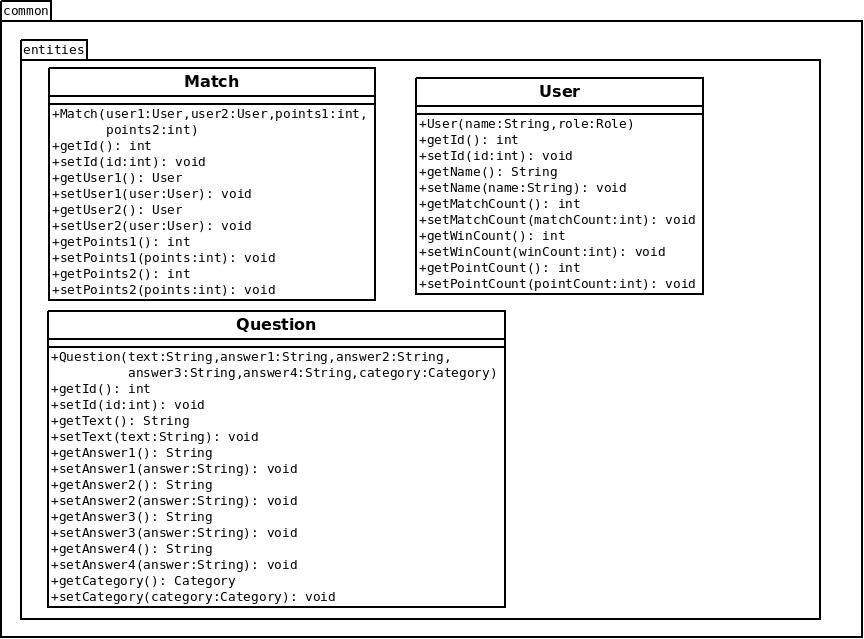
\includegraphics[width=1\textwidth]{Diagramme/entities.jpeg}
		\caption{Entities}
		\label{Entities}
	\end{minipage}
\end{figure}

\subsubsection{Net}
Das \texttt{Net}-Paket enthält eine statische Helferklasse \texttt{NetUtils}, von der Zugangsdaten des Servers abgerufen werden können und in der das Lesen und Schreiben von Sockets implementiert ist. Die Nachrichten, die über die Sockets zwischen Server und Client geschickt werden, sind durch spezielle Klassen definiert, die zur Übertragung in JSON serialisiert und nach der Übertragung deserialisiert werden, um den Informationsaustausch so einfach wie möglich zu machen. Diese Klassen unterteilen sich in \texttt{Requests} und \texttt{Responses}:

\textbf{Requests} werden von einem Client an den Server geschickt, um Daten anzufordern oder mit einem anderen Client zu kommunizieren. 

\textbf{Responses} werden vom Server an einen Client geschickt, um angeforderte Daten zu übertragen oder ihn über etwas zu benachrichtigen. 

Diagramm NetUtils

\subsection{Server}
\subsubsection{Net}
Im \texttt{Net}-Paket ist die Funktionsweise des Servers durch die Klassen \texttt{ServerDirectory} und \texttt{ServerInbox} definiert: Wird er gestartet, wird ein Thread geöffnet, auf dem eine \texttt{ServerDirectory} auf einem Port arbeitet. Die Klasse dient zur Kontaktaufnahme mit den Clients. Für jeden Client wird zudem eine \texttt{ServerInbox} eingerichtet, die - wie der Name schon sagt - als eine Art Postfach für den Server dient und ebenfalls auf einem eigenen Thread läuft. Dort wird für die gesamte Dauer der Verbindung auf Nachrichten des Clients gewartet und anschließend verarbeitet. Ebenfalls ist in der Klasse definiert, wie der Server ggf. auf diese Nachrichten antwortet.

Diagramme ServerDirectory, ServerInbox

\subsubsection{Persistence-Modul}
Die Persistence-Schnittstelle dient zum Zugriff auf die Datenbank und ist wie folgt definiert:

Diagramm IPersistence

\subsection{App-Client}
\subsubsection{Net}
Die \texttt{Client}-Klasse öffnet ein Socket zum Server und implementiert Methoden, um \texttt{Requests} an den Server zu senden. Analog zur \texttt{ServerInbox} wird auch hier ein Thread gestartet, auf dem eine \texttt{ClientInbox} läuft. Diese bearbeitet vom Server empfangene Nachrichten, indem die jeweilige Methode des Game-Moduls aufgerufen wird.

Diagramm ClientInbox

\subsubsection{Game-Modul}
Die Game-Schnittstelle definiert, welche Funktionalität die App bieten muss und beeinflusst dadurch essentiell Spielmechanik und Menüführung:

Diagramm IGame

\subsection{HTML-Client}
Beim HTML-Client beschränkt sich die Kommunikation mit dem Server auf HTTP-Anfragen. Je nachdem, auf welche Adresse zugegriffen wird, werden intern Methoden ausgeführt, um die benötigten Daten darzustellen. Im folgenden sollen deshalb den möglichen Pfaden Methoden zugeordnet werden.

\begin{table}[h]
    \begin{tabular}{|l|l|l|l|}
    \hline Pfad & Methode & Request & Parameter\\ 
    \hline /login & ~ & POST & name, password\\ 
    	\hline
    \end{tabular}
\end{table}


\section{Datensicht}
\textit{bearbeitet von: Tobias Dellert }

\label{sec:datensicht}
\textbf{Beschreibung der Datensicht}

\begin{enumerate}
	\item{\textbf{Serversystem}}
	
	Steht für das gesamte bereitgestellte System des Servers, zu dessen Aufgaben Kommunikation mit den Systemnutzern und das Speichern
	von Informationen gehört. Diese Klasse stellt keine Implementierungsklasse dar.
	
	\item{\textbf{Server}}
	
	Stellt ServerSockets für die Clients bereit. Server ist ein Teil der Klasse Serversystem.
	
	\item{\textbf{IPersistence}}
	
	Diese Klasse ist ein Interface und stellt Operationen für Data bereit.
	
	\item{\textbf{Data}}
	
	Über die Klasse Data laufen die eigentlichen Prozesse der Datenspeicherung und Nutzerkommunikation. Es besitzt Methoden, um sowohl User, als auch
	Questions zu speichern oder zu verändern und den Ausgang abgeschlosser Spiele oder Matches zu speichern.
	
	\item{\textbf{Quizapp}}
	
	Ähnlich wie die Klasse Serversystem, ist auch Quizapp keine implementierte Klasse, sondern steht für den ganzen Bereich der App und dessen Nutzer.
	In Quizapp befinden sich die Klassen Client und User und besitzt selbst eine Collection<Question> für alle Fragen, damit der Nutzer auch offline, also 
	Serversystemunabhängig spielen kann.
	
	\item{\textbf{Client}}
	
	Die Klasse Client stellt mittels eines ServerSockets eine Verbindung mit dem Serversystem durch die Bereitschaft der Sockets von der Klasse Server her.
	
	\item{\textbf{User}}
	
	In der Klasse User befinden sich alle Informationen über den entsprechenden Nutzer, wie das Serversystem und vielleicht andere Nutzer es registrieren 
	müssen oder wollen. User besitzt unter anderem das Attribut "role", wodurch entschieden wird, ob es sich bei dem Nutzer um den Admin oder einen AppNutzer handelt.
	
	\item{\textbf{IGame}}
	
	Diese Klasse ist ein Interface, welches Operationen für die Klasse QuizGame bereitstellt.
	
	\item{\textbf{Quizgame}}
	
	Diese Klasse implementiert IGame und enthält alle Operationen die für den Spiel-, Ein-/Auslog, Registrier- und Updatevorgang von seiten der App
	nötig sind. Daher ist diese Klasse ein Teil von sowohl Spielen, als auch Einloggen/..., beides Assoziationsklassen, welche für die eben genannten Vorgänge
	stehen.
	
	\item{\textbf{Match}}
	
	Die Klasse Match beinhaltet alle Daten, die für den Ablauf eines "1gegen1-Spiels" nötig sind, wie unter anderem die beiden Namen der Spieler, sowie deren momentante Punktzahl usw.
	
	\item{\textbf{Question}}
	
	Diese Klasse beinhalten alle Daten, die für jede Frage benötigt wird, wie ihren Text, ihre Kategorie und zur Auswahl stehenden Antowrten auf die Frage an sich.
	
	\item{\textbf{Spielen}}
	
	Diese Assoziationsklasse steht für den Spielvorgang und benötigt daher die Klassen Question und Match. 
	
	\item{\textbf{Einloggen/Ausloggen/Registrieren/Update}}
	
	Diese Assoziationsklassen steht für die in dessen Namen stehenden Vorgänge und beschreibt damit eine der Relationen von Quizapp und Serversystem.
	
	\item{\textbf{Bearbeiten/Hinzufügen/Löschen}}
	
	Diese Assoziationsklasse beschreibt die Relation der Klasse User in der Rolle des Admin und	Serversystem. Der Admin soll Fragen und Nutzer berarbeiten, löschen 
	oder hinzufügen können.
	
\end{enumerate}

\section{Ausführungssicht}
\textit{bearbeitet von: Daniel Pupat }

\label{sec:ausfuehrung}

{\it
Die Ausführungssicht beschreibt das Laufzeitverhalten. Hier
werden die Laufzeitelemente aufgeführt und beschrieben, welche Module
sie zur Ausführung bringen. Ein Modul kann von mehreren
Laufzeitelementen zur Laufzeit verwendet werden. Die Ausführungssicht
beschreibt darüber hinaus, welche Laufzeitelemente spezifisch
miteinander kommunizieren. Zudem wird bei verteilten Systemen
(z.B. Client-Server-Systeme) dargestellt, welche Module von welchen
Prozessen auf welchen Rechnern ausgeführt werden.}


%Der Name zu korregieren hier?
\section[Zusammenhänge zwischen Anwendungsfällen und Architektur]{Zusammenhänge zwischen Anwendungsfällen und Architektur\sectionmark{Zusammenhänge AF u. Architektur}}
\sectionmark{Zusammenhänge AF u. Architektur}
\textit{bearbeitet von: }

\label{sec:anwendungsfaelle}

{\it In diesem Abschnitt sollen Sequenzdiagramme mit Beschreibung(!)
  für \variante{zwei bis drei von Euch ausgewählte
    Anwendungsfälle}{einen von Euch ausgewählten Anwendungsfall}
  erstellt werden. Ein Sequenzdiagramm beschreibt den
  Nachrichtenverkehr zwischen allen Modulen, die an der Realisierung
  des Anwendungsfalles beteiligt sind.  \variante{Wählt die
    Anwendungsfälle so, dass nach Möglichkeit alle Module Eures
    entworfenen Systems in mindestens einem Sequenzdiagramm
    vorkommen. Falls Euch das nicht gelingt, versucht möglichst viele
    und die wichtigsten Module abzudecken.}{Dazu könnt ihr Euch einen
    Anwendungsfall heraussuchen, der möglichst viele Module der
    Architektur abdeckt. In SWP-2 werden wir mehrere Anwendungsfälle
    betrachten und eine umfangreichere Abdeckung der Architektur
    anstreben.} }




\section{Evolution}
\textit{bearbeitet von: Tim Ellhoff }

\label{sec:evolution}

In diesem Abschnitt geht es um mögliche Änderungen, Anpassungen bzw. Erweiterungen, die vorgenommen werden müssten, wenn sich Anforderungen des Systems ändern. \\
Dabei ist wichtig, dass sich solche Änderungen möglichst modular realisieren lassen, ohne die bestehende Architektur komplett zu verändern, was sehr aufwändig und somit nicht wünschenswert wäre. \\
Im Folgenden werden einige wichtige mögliche neue Anforderungen bzw. Erweiterungen aufgelistet und deren jeweiligen zu implementierenden Änderungen an der Architektur beschrieben. 


\subsection*{Erweiterungsmöglichkeiten}

Da sich aus der Anforderungsspezifikation im Abschnitt ''Ausblick'' noch keine genauen absehbaren Änderungen ergeben haben, werden im Folgenden potenzielle Änderungen aufgezeigt, die näher beschrieben werden.

\subsubsection*{1. Erweiterung des GUI-Layouts}

Es wäre möglicherweise wünschenswert, wenn man als Benutzer nicht nur ein GUI-Design in der Quiz-App verwenden könnte, sondern mehrere. Dafür müsste eine Funktionalität hinzugefügt werden, um zwischen verschiedenen Benutzeroberflächen wählen zu können (z.B. verschiedene Themes oder Farbwahlen). \\
Dazu müssten entsprechende Referenzierungen von neuen GUI-Style-Änderungen mit Bilddateien stattfinden sowie für Textanpassungen die XML-Dateien im entsprechendem Paket verändert bzw. erweitert werden. 

\subsubsection*{2. Mehrsprachigkeit}

Auch wenn die Mindestanforderungen keine Mehrsprachigkeit für die Quizapp vorschreibt, wäre es ggf. wünschenswert, dass die Möglichkeit besteht, mehrere Sprachen für die Quiz-App zu unterstützen, um einen größeren bzw. internationaleren Spielerkreis anzusprechen. Insofern wäre es denkbar, dass neben Deutsch eine weitere Sprache eingebaut werden könnte. Englisch würde sich natürlich anbieten.



\end{document}


%%% Local Variables: 
%%% mode: latex
%%% mode: reftex
%%% mode: flyspell
%%% ispell-local-dictionary: "de_DE"
%%% TeX-master: t
%%% End: 
